% =====================================================================
\chapter{Derivadas parciales, gradiente y regla de la cadena}
\label{tema:4}
% =====================================================================

La derivada de una función de una variable mide cuánto cambia la función por unidad de cambio de la variable. Con varias variables hay que elegir \emph{en qué dirección} se mueve uno. Las derivadas parciales miden el cambio en las direcciones de los ejes; el gradiente las reúne en un vector que apunta hacia donde la función crece más deprisa y que es perpendicular a las curvas de nivel. Este es el objeto central del entrenamiento de redes neuronales. La presentación sigue las sesiones~26--27 y~32--38 de 18.02SC~\cite{mit1802}, las §4.3--4.6 de OpenStax~\cite{openstax3}, los capítulos~13 de Strang~\cite{strangcalc} y~8 de Apostol~\cite{apostol2}.

\section{Derivadas parciales}

\begin{definicion}[Derivadas parciales]\label{def:parcial}
Sea $f$ una función de $(x,y)$ definida cerca de $(a,b)$. Las \emph{derivadas parciales} de $f$ en $(a,b)$ son
\begin{align*}
f_x(a,b)&=\pd fx(a,b)=\lim_{h\to0}\frac{f(a+h,b)-f(a,b)}{h},\\
f_y(a,b)&=\pd fy(a,b)=\lim_{h\to0}\frac{f(a,b+h)-f(a,b)}{h},
\end{align*}
cuando existen. Para tres o más variables la definición es análoga.
\end{definicion}

Para calcular $f_x$ se deriva respecto de $x$ tratando $y$ como una constante, con todas las reglas de una variable. Geométricamente, $f_x(a,b)$ es la pendiente de la curva que se obtiene al cortar la gráfica con el plano vertical $y=b$.

\begin{ejemplo}\label{ej:t4-parciales}
Sea $f(x,y)=x^2y+y^3$. Entonces $f_x=2xy$ y $f_y=x^2+3y^2$. En $(1,2)$: $f(1,2)=10$, $f_x(1,2)=4$ y $f_y(1,2)=13$. Las derivadas segundas son $f_{xx}=2y$, $f_{yy}=6y$ y $f_{xy}=(f_x)_y=2x=(f_y)_x=f_{yx}$.
\end{ejemplo}

La igualdad de las derivadas cruzadas del ejemplo no es casual.

\begin{teorema}[Schwarz]\label{teo:schwarz}
Si $f_{xy}$ y $f_{yx}$ existen y son continuas en un entorno de $(a,b)$, entonces $f_{xy}(a,b)=f_{yx}(a,b)$.
\end{teorema}

La demostración, que usa dos veces el teorema del valor medio, puede consultarse en Apostol~\cite[cap.~8]{apostol2}. Todas las funciones de este módulo construidas con polinomios, exponenciales, logaritmos y funciones trigonométricas cumplen la hipótesis en el interior de su dominio.

\section{Diferenciabilidad y plano tangente}

La mera existencia de las derivadas parciales es una condición débil: solo informa de lo que ocurre sobre dos rectas. La noción adecuada exige que $f$ se parezca a una función afín en \emph{todas} las direcciones.

\begin{definicion}[Diferenciabilidad]\label{def:diferenciable}
Una función $f$ definida cerca de $\va\in\R^n$ es \emph{diferenciable} en $\va$ si existe un vector $\mathbf g\in\R^n$ tal que
\[
\lim_{\mathbf h\to\vcero}\frac{f(\va+\mathbf h)-f(\va)-\mathbf g\cdot\mathbf h}{\norm{\mathbf h}}=0 .
\]
Es decir, $f(\va+\mathbf h)=f(\va)+\mathbf g\cdot\mathbf h+\varepsilon(\mathbf h)\norm{\mathbf h}$ con $\varepsilon(\mathbf h)\to0$.
\end{definicion}

\begin{teorema}\label{teo:diferenciable}
Si $f$ es diferenciable en $\va$, entonces:
\begin{enumerate}
  \item $f$ es continua en $\va$;
  \item existen las derivadas parciales en $\va$ y $\mathbf g=\nabla f(\va)$, donde el \emph{gradiente} es el vector $\nabla f(\va)=\bigl(f_{x_1}(\va),\dots,f_{x_n}(\va)\bigr)$.
\end{enumerate}
\end{teorema}

\begin{proof}
(i) En la igualdad de la \cref{def:diferenciable}, cuando $\mathbf h\to\vcero$ se tiene $\abs{\mathbf g\cdot\mathbf h}\le\norm{\mathbf g}\norm{\mathbf h}\to0$ por Cauchy--Schwarz y $\varepsilon(\mathbf h)\norm{\mathbf h}\to0$, luego $f(\va+\mathbf h)\to f(\va)$. (ii) Tómese $\mathbf h=h\mathbf e_i$, con $\mathbf e_i$ el $i$-ésimo vector de la base canónica y $h\to0$. Entonces $\mathbf g\cdot\mathbf h=g_ih$ y
\[
\frac{f(\va+h\mathbf e_i)-f(\va)}{h}=g_i+\varepsilon(h\mathbf e_i)\frac{\abs h}{h}\longrightarrow g_i,
\]
de modo que $f_{x_i}(\va)$ existe y vale $g_i$.
\end{proof}

El recíproco de (ii) es falso (\cref{eje:4-no-diferenciable}). Una condición suficiente práctica es la siguiente, cuya demostración puede verse en Apostol~\cite[cap.~8]{apostol2}: \emph{si las derivadas parciales de $f$ existen y son continuas en un entorno de $\va$, entonces $f$ es diferenciable en $\va$.}

\begin{definicion}[Plano tangente y aproximación lineal]\label{def:tangente}
Si $f$ es diferenciable en $(a,b)$, el \emph{plano tangente} a la gráfica de $f$ en $(a,b,f(a,b))$ es
\[
z=f(a,b)+f_x(a,b)(x-a)+f_y(a,b)(y-b),
\]
y la \emph{aproximación lineal} es $f(a+\Delta x,b+\Delta y)\approx f(a,b)+f_x(a,b)\Delta x+f_y(a,b)\Delta y$. Con notación de diferenciales, $df=f_x\,dx+f_y\,dy$.
\end{definicion}

\begin{ejemplo}\label{ej:t4-aproximacion}
Sea $f(x,y)=\sqrt{x^2+y^2}$ en $(3,4)$: $f=5$, $f_x=x/f=\tfrac35$ y $f_y=y/f=\tfrac45$. El plano tangente es $z=5+\tfrac35(x-3)+\tfrac45(y-4)=\tfrac{3x+4y}{5}$. Para estimar $\sqrt{3{,}02^2+3{,}97^2}$ se toman $\Delta x=0{,}02$ y $\Delta y=-0{,}03$: $5+0{,}012-0{,}024=4{,}988$, frente al valor exacto $4{,}98812$.
\end{ejemplo}

\section{Regla de la cadena}

\begin{teorema}[Regla de la cadena]\label{teo:cadena}
Sea $\vr(t)=(x(t),y(t))$ derivable en $t_0$ y $f$ diferenciable en $\vr(t_0)$. Entonces $w(t)=f(\vr(t))$ es derivable en $t_0$ y
\[
\frac{dw}{dt}=f_x\frac{dx}{dt}+f_y\frac{dy}{dt}=\nabla f(\vr(t_0))\cdot\vr\,'(t_0).
\]
\end{teorema}

\begin{proof}
Sea $\mathbf h=\vr(t_0+s)-\vr(t_0)$, que tiende a $\vcero$ cuando $s\to0$. Por la diferenciabilidad de $f$,
\[
\frac{w(t_0+s)-w(t_0)}{s}=\nabla f(\vr(t_0))\cdot\frac{\mathbf h}{s}+\varepsilon(\mathbf h)\frac{\norm{\mathbf h}}{s}.
\]
Cuando $s\to0$, $\mathbf h/s\to\vr\,'(t_0)$, de modo que el primer sumando tiende a $\nabla f\cdot\vr\,'(t_0)$; en el segundo, $\norm{\mathbf h}/\abs s\to\norm{\vr\,'(t_0)}$ está acotado y $\varepsilon(\mathbf h)\to0$. (Si $\mathbf h=\vcero$ para algún $s$, se toma $\varepsilon(\vcero)=0$ y la igualdad sigue valiendo.)
\end{proof}

Si $x$ e $y$ dependen de dos variables $(u,v)$, se aplica el teorema fijando una de ellas:
\begin{equation}\label{eq:t4-cadena2}
\pd wu=\pd wx\pd xu+\pd wy\pd yu,\qquad \pd wv=\pd wx\pd xv+\pd wy\pd yv .
\end{equation}
La regla se recuerda con un \emph{diagrama de árbol}: cada camino de $w$ a la variable final aporta el producto de las derivadas de sus tramos, y se suman las aportaciones de todos los caminos.

\begin{figure}[ht]
\centering
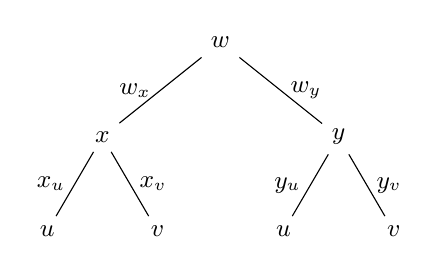
\begin{tikzpicture}[font=\small,level distance=1.2cm,
  level 1/.style={sibling distance=3cm},level 2/.style={sibling distance=1.4cm}]
  \node {$w$}
    child {node {$x$} child {node {$u$} edge from parent node[left] {$x_u$}} child {node {$v$} edge from parent node[right] {$x_v$}} edge from parent node[left] {$w_x$}}
    child {node {$y$} child {node {$u$} edge from parent node[left] {$y_u$}} child {node {$v$} edge from parent node[right] {$y_v$}} edge from parent node[right] {$w_y$}};
\end{tikzpicture}
\caption{Diagrama de árbol de $w=f(x,y)$ con $x=x(u,v)$, $y=y(u,v)$. Los dos caminos de $w$ a $u$ dan $w_u=w_xx_u+w_yy_u$.}
\label{fig:t4-arbol}
\end{figure}

\begin{ejemplo}\label{ej:t4-polares}
Sea $w=x^2+y^2$ con $x=r\cos\theta$, $y=r\sin\theta$. Por~\eqref{eq:t4-cadena2}, $w_r=2x\cos\theta+2y\sin\theta=2r$ y $w_\theta=2x(-r\sin\theta)+2y(r\cos\theta)=0$, como corresponde a $w=r^2$, que no depende de $\theta$.
\end{ejemplo}

\section{Gradiente y derivada direccional}

\begin{definicion}[Derivada direccional]\label{def:direccional}
Sea $\vu$ un vector \emph{unitario}. La \emph{derivada direccional} de $f$ en $\va$ según $\vu$ es
\[
D_{\vu}f(\va)=\lim_{t\to0}\frac{f(\va+t\vu)-f(\va)}{t},
\]
la tasa de cambio de $f$ por unidad de longitud recorrida en la dirección de $\vu$. Para $\vu=\vi$ y $\vu=\vj$ se obtienen $f_x$ y $f_y$.
\end{definicion}

\begin{teorema}[Cálculo de la derivada direccional]\label{teo:direccional}
Si $f$ es diferenciable en $\va$, entonces $D_{\vu}f(\va)=\nabla f(\va)\cdot\vu$ para todo vector unitario $\vu$.
\end{teorema}

\begin{proof}
Es la regla de la cadena (\cref{teo:cadena}) aplicada a la recta $\vr(t)=\va+t\vu$, cuya velocidad es $\vr\,'(0)=\vu$.
\end{proof}

\begin{corolario}[Dirección de máximo crecimiento]\label{cor:maximo-crecimiento}
Sea $\nabla f(\va)\neq\vcero$. Entre todas las direcciones unitarias, $D_{\vu}f(\va)$ alcanza su máximo, $\norm{\nabla f(\va)}$, para $\vu=\nabla f(\va)/\norm{\nabla f(\va)}$, su mínimo, $-\norm{\nabla f(\va)}$, en la dirección opuesta, y se anula en las direcciones perpendiculares al gradiente.
\end{corolario}

\begin{proof}
Por Cauchy--Schwarz (\cref{teo:cs}), $\abs{\nabla f\cdot\vu}\le\norm{\nabla f}\norm{\vu}=\norm{\nabla f}$, con igualdad si y solo si $\vu$ es múltiplo de $\nabla f$; los dos múltiplos unitarios dan $\pm\norm{\nabla f}$. Además $\nabla f\cdot\vu=\norm{\nabla f}\cos\theta$ es nulo exactamente cuando $\theta=\pi/2$.
\end{proof}

\begin{teorema}[El gradiente es normal a los conjuntos de nivel]\label{teo:gradiente-normal}
Sea $f$ diferenciable y $\vr(t)$ una curva derivable contenida en el conjunto de nivel $f=c$, con $\vr(t_0)=\va$. Entonces $\nabla f(\va)\cdot\vr\,'(t_0)=0$.
\end{teorema}

\begin{proof}
Como $f(\vr(t))=c$ para todo $t$, al derivar con la regla de la cadena se obtiene $0=\frac{d}{dt}f(\vr(t))=\nabla f(\vr(t))\cdot\vr\,'(t)$, y basta evaluar en $t_0$.
\end{proof}

En consecuencia, el \emph{plano tangente} a la superficie de nivel $F(x,y,z)=c$ en un punto $P_0$ con $\nabla F(P_0)\neq\vcero$ es el plano de normal $\nabla F(P_0)$: $\nabla F(P_0)\cdot(X-P_0)=0$. El plano tangente a una gráfica $z=f(x,y)$ es el caso particular $F(x,y,z)=f(x,y)-z$.

\begin{ejemplo}\label{ej:t4-direccional}
Para $f(x,y)=x^2y+y^3$ en $(1,2)$, $\nabla f=(4,13)$. En la dirección $\vu=(3,4)/5$, $D_{\vu}f=(12+52)/5=12{,}8$. La tasa máxima es $\norm{\nabla f}=\sqrt{185}\approx13{,}60$, en la dirección $(4,13)/\sqrt{185}$, y $f$ no varía, a primer orden, en las direcciones $\pm(13,-4)/\sqrt{185}$, tangentes a la curva de nivel $f=10$.
\end{ejemplo}

\begin{observacion}[Errores frecuentes]
\begin{enumerate}[label=(\alph*)]
\item La fórmula $D_{\vu}f=\nabla f\cdot\vu$ exige $\norm{\vu}=1$. Si la dirección viene dada por un vector $\vw$ cualquiera, hay que normalizarlo: $\vu=\vw/\norm{\vw}$.
\item El gradiente de $f(x,y)$ es un vector del plano $xy$ (del dominio), no de la superficie gráfica; es perpendicular a las curvas de nivel, no a la gráfica.
\item La existencia de derivadas parciales no garantiza la diferenciabilidad, ni siquiera la continuidad (\cref{eje:4-no-diferenciable}).
\item En la regla de la cadena hay que sumar las contribuciones de todos los caminos del árbol; omitir uno es el error más común.
\end{enumerate}
\end{observacion}

\begin{observacion}[Conexión con el curso]
El \cref{cor:maximo-crecimiento} es el fundamento del \emph{descenso de gradiente} $\mathbf w_{k+1}=\mathbf w_k-\eta\nabla L(\mathbf w_k)$ (módulo~7): cada paso se mueve en la dirección en que la pérdida $L$ decrece más deprisa. La regla de la cadena aplicada sistemáticamente a una composición de muchas funciones es la \emph{retropropagación} (módulo~10), y su forma matricial, con el jacobiano, se estudia en el módulo~4 (temas~1 y~2). El gradiente de la log-suma-exp es la softmax (\cref{eje:4-softmax}), lo que explica la sencillez del gradiente de la entropía cruzada (módulo~8).
\end{observacion}

\begin{lecturas}
\item MIT 18.02SC~\cite{mit1802}, unidad~2, parte~A, sesiones~26--27 (derivadas parciales, aproximación), y parte~B, sesiones~32--38 (diferenciales, regla de la cadena, gradiente, derivada direccional).
\item OpenStax \emph{Calculus}, vol.~3~\cite{openstax3}, §4.3 «Partial Derivatives», §4.4 «Tangent Planes and Linear Approximations», §4.5 «The Chain Rule» y §4.6 «Directional Derivatives and the Gradient».
\item Strang, \emph{Calculus}~\cite{strangcalc}, §13.2--13.5.
\item Apostol~\cite{apostol2}, cap.~8, para las demostraciones del teorema de Schwarz y de la condición suficiente de diferenciabilidad.
\end{lecturas}

\section*{Ejercicios del tema 4}
\addcontentsline{toc}{section}{Ejercicios del tema 4}

\begin{ejercicio}{1}{eje:4-conceptos}
Razone si son verdaderas o falsas: (a) $f_x(a,b)$ es la pendiente del corte de la gráfica con el plano $x=a$; (b) si $\nabla f(\va)=(3,4)$, la derivada de $f$ en la dirección de $\vw=(1,1)$ es $7$; (c) si $f$ tiene derivadas parciales en $\va$, es continua en $\va$; (d) si $\nabla f(\va)\neq\vcero$, la recta tangente en $\va$ a la curva de nivel que pasa por $\va$ es perpendicular a $\nabla f(\va)$.
\end{ejercicio}

\begin{ejercicio}{2}{eje:4-parciales}
Calcule las derivadas parciales primeras de: (a) $x^3y-3xy^2+2y^2$; (b) $x^2/y$; (c) $\sin(3x+2y)$; (d) $e^{xy}$; (e) $x\ln(2x+y)$; (f) $x^2z-2yz^3$.
\fuente{adaptado de MIT 18.02SC~\cite{mit1802}, problemas suplementarios, 2A-2.}
\end{ejercicio}

\begin{ejercicio}{2}{eje:4-schwarz}
Compruebe que $f_{xy}=f_{yx}$ para: (a) $x^my^n$, con $m,n$ enteros positivos; (b) $\cos(x^2+y)$; (c) $f(x)g(y)$, con $f,g$ derivables dos veces. (d) Compruebe también que $w=e^{ax}\sin(ay)$ satisface la ecuación de Laplace $w_{xx}+w_{yy}=0$.
\fuente{adaptado de MIT 18.02SC~\cite{mit1802}, problemas suplementarios, 2A-3 y 2A-5.}
\end{ejercicio}

\begin{ejercicio}{2}{eje:4-tangente}
Halle el plano tangente a la gráfica de: (a) $z=xy^2$ en $(1,1,1)$; (b) $z=e^{x}\cos y$ en $(0,0,1)$. Use (b) para aproximar $e^{0{,}1}\cos(0{,}1)$ y compare con el valor exacto.
\fuente{adaptado de MIT 18.02SC~\cite{mit1802}, problemas suplementarios, 2B-1 y 2B-5.}
\end{ejercicio}

\begin{ejercicio}{2}{eje:4-aproximacion}
(a) Los catetos de un triángulo rectángulo miden $3$ y $4$ y cada uno aumenta $0{,}01$. Estime con la aproximación lineal el cambio de la hipotenusa. (b) Una caja mide $5\times10\times20$~cm y cada medida tiene un error posible de $\pm0{,}1$~cm. Estime con diferenciales el error posible del volumen.
\fuente{adaptado de MIT 18.02SC~\cite{mit1802}, problemas suplementarios, 2B-3 y 2C-2.}
\end{ejercicio}

\begin{ejercicio}{2}{eje:4-gradiente}
Halle el gradiente en $P$ y la derivada direccional en $P$ en la dirección del vector $\va$: (a) $f=x^3+2y^3$, $P=(1,1)$, $\va=\vi-\vj$; (b) $w=xy/z$, $P=(2,-1,1)$, $\va=\vi+2\vj-2\vk$.
\fuente{adaptado de MIT 18.02SC~\cite{mit1802}, problemas suplementarios, 2D-1.}
\end{ejercicio}

\begin{ejercicio}{2}{eje:4-max-direccional}
Para $w=\ln(4x-3y)$ en $(1,1)$, halle: (a) el máximo y el mínimo de la derivada direccional y las direcciones en que se alcanzan; (b) las direcciones en que la derivada direccional es nula.
\fuente{adaptado de MIT 18.02SC~\cite{mit1802}, problemas suplementarios, 2D-2.}
\end{ejercicio}

\begin{ejercicio}{2}{eje:4-tangente-nivel}
Halle el plano tangente a la superficie, vista como superficie de nivel, en el punto indicado: (a) $xy^2z^3=12$ en $(3,2,1)$; (b) el elipsoide $x^2+4y^2+9z^2=14$ en $(1,1,1)$.
\fuente{adaptado de MIT 18.02SC~\cite{mit1802}, problemas suplementarios, 2D-3.}
\end{ejercicio}

\begin{ejercicio}{2}{eje:4-cadena-t}
Calcule $dw/dt$ de dos maneras, con la regla de la cadena y sustituyendo antes de derivar: (a) $w=xyz$ con $x=t$, $y=t^2$, $z=t^3$; (b) $w=x^2-y^2$ con $x=\cos t$, $y=\sin t$.
\fuente{adaptado de MIT 18.02SC~\cite{mit1802}, problemas suplementarios, 2E-1.}
\end{ejercicio}

\begin{ejercicio}{2}{eje:4-cadena-uv}
Sea $w=f(x,y)$ con $\nabla f(0,1)=(2,3)$, y sean $x=u^2-v^2$, $y=uv$. Calcule $\partial w/\partial u$ y $\partial w/\partial v$ en $(u,v)=(1,1)$.
\fuente{adaptado de MIT 18.02SC~\cite{mit1802}, problemas suplementarios, 2E-4.}
\end{ejercicio}

\begin{ejercicio}{2}{eje:4-softmax}
Sea $f(x,y)=\ln(e^x+e^y)$. (a) Demuestre que $\nabla f=(\sigma_1,\sigma_2)$ con $\sigma_1=\dfrac{e^x}{e^x+e^y}$, $\sigma_2=\dfrac{e^y}{e^x+e^y}$, y que $\sigma_1,\sigma_2\in(0,1)$ con $\sigma_1+\sigma_2=1$. (b) Calcule la derivada direccional en la dirección $(1,1)/\sqrt2$ y explique el resultado a partir de $f(x+t,y+t)$. (c) Aproxime linealmente $f(1{,}1;\,-0{,}1)$ desde $(1,0)$ y compare con el valor exacto.
\end{ejercicio}

\begin{ejercicio}{3}{eje:4-polares}
Sea $w=f(x,y)$ diferenciable, con $x=r\cos\theta$, $y=r\sin\theta$ y $r>0$. Demuestre que
\[
w_x^2+w_y^2=w_r^2+\frac{1}{r^2}w_\theta^2 .
\]
\fuente{adaptado de MIT 18.02SC~\cite{mit1802}, problemas suplementarios, 2E-5.}
\end{ejercicio}

\begin{ejercicio}{3}{eje:4-euler}
(a) Sea $f$ derivable en una variable y $w=f(y/x)$ para $x\neq0$. Demuestre que $xw_x+yw_y=0$. (b) Una función $g(x,y)$ es \emph{homogénea de grado $k$} si $g(tx,ty)=t^kg(x,y)$ para todo $t>0$. Demuestre que, si es diferenciable, cumple la \emph{identidad de Euler} $xg_x+yg_y=k\,g$. (c) Compruébela para $g=x^2y+y^3$.
\fuente{adaptado de MIT 18.02SC~\cite{mit1802}, problemas suplementarios, 2E-8.}
\end{ejercicio}

\begin{ejercicio}{3}{eje:4-material}
Sea $f(x,y,z,t)$ diferenciable y $\vr(t)=(x(t),y(t),z(t))$ la trayectoria de una partícula, con velocidad $\vv=\vr\,'(t)$. Sea $\nabla f$ el gradiente respecto de las variables espaciales. Demuestre que la \emph{derivada material} $\frac{Df}{Dt}=\frac{d}{dt}f(\vr(t),t)$ vale
\[
\frac{Df}{Dt}=\pd ft+\vv\cdot\nabla f .
\]
\fuente{adaptado de MIT 18.02SC~\cite{mit1802}, \emph{problem set}~5, parte~II, problema~2.}
\end{ejercicio}

\begin{ejercicio}{3}{eje:4-no-diferenciable}
Sea $f(x,y)=\dfrac{xy}{x^2+y^2}$ si $(x,y)\neq(0,0)$ y $f(0,0)=0$. (a) Demuestre que $f_x(0,0)$ y $f_y(0,0)$ existen y valen~$0$. (b) Demuestre que $f$ no es diferenciable en el origen. (c) Calcule, para $\vu=(1,1)/\sqrt2$, el cociente $\bigl(f(t\vu)-f(\vcero)\bigr)/t$ y explique por qué la derivada direccional $D_{\vu}f(\vcero)$ no existe, aunque $\nabla f(\vcero)\cdot\vu=0$.
\end{ejercicio}
